
\section{3D Push-Pull is NP-hard}
\label{3DNPhard}
In this section we prove that 3D Push-$k$ Pull-$l$ with fixed blocks is NP-hard, for all positive $k$ and $l$. All of the hard work was done in Section~\ref{2DNPhard}. Here we will simply show how we can use the additional dimension to tweak the previous gadgets to build them without thin walls. We reduce from 3SAT, constructing our variables from chains of 3D Set-Verify gadgets, and our clauses from the verify side of the corresponding 3D Set-Verify gadget.

\begin{theorem}
3D Push-$k$ Pull-$l$ with fixed blocks is NP-hard, for all positive $k$ and $l$.
\end{theorem}
\begin{proof}
We follow the proof of Theorem~\ref{thm:2DNPhard} using a modified Set-Verify gadget, shown in Figure~\ref{fig:3DSetVerify}.  It can be easily checked that this has the same properties as the Set-Verify given in Section~\ref{sec:SetVerifyGadgets}. The cyclic ordering of the entrances in the 3D Set-Verify is different from that of the 2D Set-Verify, however this is not important as we no longer need to construct crossovers. Also, this construction does not use thin-walls. While this was critical in the prior construction due to the need for closely packed turns, the additional dimension allows enough freedom to keep separate hallways from being adjacent to each other. With a functional Set-Verify gadget, the remaining constructions of variables and clauses proceeded as in Section \ref{sec:2DPushPull3SAT}. No crossover gadgets are needed since we are working in 3D. Finally, we note that all blocks are in hallways of length at most 3, thus the gadgets still function as described for any positive push and pull values.

\begin{wrapfigure}{hr}{0.45\textwidth}
\vspace{-5mm}
  \centering
%  \begin{figure}[t]
%    \centering
    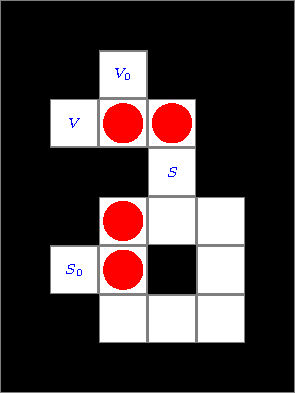
\includegraphics[width=.4\textwidth]{SetVerify3D}
    \caption{A Set-Verify gadget in 3D where the entrances and exits extend upward, notated by the diagonal arrows. This gadget is in the unset state.}
    \label{fig:3DSetVerify}
    \vspace{-12mm}
\end{wrapfigure}

%As before, in the unset state the only possible traversal is $S_i$ to $S_0$. This traversal allows the top right bock to be pulled down, moving the gadget into the set state. From here the $V$ to $V_0$ traversal is possible, as well as going back through the $S_0$ to $S$ pathway. However, the $S$ to $S_0$ traversal is not possible.

%Variables are composed of hallways of 3D Set-Verify gadgets connected $S_0$ to $S$, one for each clause in which the variable appears, as in Figure~\ref{fig:NPVariableGadget}. Clauses are composed of three 3D Set-Verify gadgets connected in parallel as in Figure~\ref{fig:NPClauseGadget}. The details of these constructions follow those in Section~\ref{sec:2DPushPull3SAT} This completes the reduction from 3SAT. In addition, we note that all blocks are in hallways of length at most 3, thus the gadgets still function as described for any positive push and pull values.
\end{proof}




